\documentclass[11pt,a4paper]{article}

% --- Core Packages ---
\usepackage[utf8]{inputenc}
\usepackage[T1]{fontenc}
\usepackage{lmodern}
\usepackage[margin=1in]{geometry}
\usepackage{amsmath,amssymb,amsfonts}
\usepackage{booktabs}
\usepackage{longtable}
\usepackage{tabularx}
\usepackage{xltabular}
\usepackage{array}
\usepackage{graphicx}
\usepackage{caption}
\usepackage{subcaption}
\usepackage{hyperref}
\usepackage{xcolor}
\usepackage{enumitem}

\hypersetup{
    colorlinks=true,
    linkcolor=blue!70!black,
    citecolor=blue!70!black,
    urlcolor=teal!70!black
}

\title{\textbf{Manuscript Architecture \& Detailed Outline: \\ Scalable GeoAI for Mapping and Explaining Micro-Scale Physical Living Standards and Spatial Segregation}}

\author{
    \textbf{Dimas Rizqi Dwiaji} \\
    Scalable Earth \\
}

\date{\today}

\begin{document}

\maketitle

\begin{abstract}
Placeholder...
\end{abstract}

\noindent\textbf{Keywords:} Placeholder...

\vspace{1em}
\hrule
\vspace{1.5em}

\section{Introduction}
\subsection{Problem Statement and Context}
\begin{itemize}[leftmargin=*]
    \item \textbf{Spatial Granularity and Aggregation Mismatch}
    \begin{itemize}
        \item Living standard disparities occur locally, where contrasting housing conditions and informal settlements exist adjacent to planned developments within hundreds of meters.
        \item Standard inequality measures, such as the Gini coefficient and official poverty rates, aggregate data to municipal or district levels.
        \item Spatial aggregation (MAUP) smooths local variations, masking intra-municipal disparities and localized segregation.
    \end{itemize}
    \item \textbf{Cross-Regional Comparability Gap}
    \begin{itemize}
        \item Existing neighborhood-level assessments rely on localized surveys and municipal administrative records.
        \item Disparate survey definitions, census boundaries, and collection intervals hinder standardized comparisons of localized disparity across cities and countries.
        \item Standardized cross-regional comparisons require consistent, continuously available measurement frameworks.
    \end{itemize}
    \item \textbf{Administrative Data Scarcity and Open Geospatial Data}
    \begin{itemize}
        \item Emerging economies and rapidly urbanizing regions frequently face administrative data gaps, including incomplete cadastral records and unmapped settlements.
        \item Frameworks reliant on detailed municipal registers cannot scale to data-sparse regions.
        \item Global Earth observation records (Sentinel, Landsat, atmospheric reanalysis) and open spatial geometry datasets (open building heights, street networks, POIs) provide uniform, continuous physical measurements across metropolitan areas without relying on local administrative capacity.
    \end{itemize}
    \item \textbf{Non-Linear Indicator Interaction and the Need for Unsupervised Learning}
    \begin{itemize}
        \item Physical indicators (such as building density, living area per capita, surface temperature, and street network access) exhibit non-linear interactions across urban space (for example, high building density reflects different living standards depending on floor area and tree cover).
        \item Comprehensive, continuous ground-truth labels for composite living conditions and segregation boundaries do not exist across metropolitan areas.
        \item Because supervised training targets are unavailable across continuous space, identifying how these non-linear indicators group into cohesive living standard typologies requires unsupervised representation learning.
        \item A spatial graph neural network learns latent representations directly from the multi-channel indicators and spatial adjacency without requiring training labels.
    \end{itemize}
\end{itemize}

\subsection{Research Questions}
\begin{itemize}[leftmargin=*]
    \item \textbf{RQ1}: How can open Earth observation data and open spatial geometries be formulated into an absolute physical living standard index that is continuous and comparable across administrative boundaries?
    \item \textbf{RQ2}: How can unsupervised spatial graph representation learning capture non-linear indicator interactions to identify latent physical living typologies and spatial segregation boundaries without ground-truth labels?
    \item \textbf{RQ3}: To what extent do the unsupervised physical living typologies and segregation boundaries align with local ground-truth deprivation surveys (such as KOTAKU slum registries), and how do they compare with satellite-derived asset wealth estimates?
\end{itemize}

\section{Literature Review and Theoretical Framework}
\begin{itemize}[leftmargin=*]
    \item \textbf{Remote Sensing and Machine Learning Wealth Prediction}: Evolution from nighttime lights transfer learning to multi-source gradient-boosted trees; distinction between volatile monthly consumption expenditure and persistent structural physical capital.
    \item \textbf{Urban Morphology and Slum Detection}: UN-Habitat shelter deprivation criteria ($<9.0\text{ m}^2$ overcrowding, structural durability, improved sanitation); breakthroughs in open 3D building volume extraction.
    \item \textbf{15-Minute City Accessibility and \texttt{city2graph}}: Cumulative opportunities vs. gravity accessibility; shift to Overture Maps GERS; necessity of topological street network isochrones over Euclidean circular buffers in capturing wall severance.
    \item \textbf{Graph Neural Networks in Urban Spatial Modeling}: GCN and GAT architectures; the DOMINANT framework for graph anomaly detection; spatial autocorrelation baselines (LISA).
    \item \textbf{The 4-Quadrant Divergence Framework}: Theoretical formulation of Asset Wealth vs. In-Situ Physical Living Standards.
\end{itemize}

\section{Study Area and Dataset}

\subsection{Study Area: Greater Jakarta (Jabodetabek) and Karawang Corridor}
The empirical investigation is situated across the Greater Jakarta metropolitan agglomeration (\textit{Jabodetabek}) and the contiguous industrial corridor of Karawang Regency in West Java, Indonesia (Figure~\ref{fig:study_area_map}). Spatial extent covers approximately $9,800\text{ km}^2$ ($[106.35^\circ\text{E}, -6.75^\circ\text{S}]$ to $[107.65^\circ\text{E}, -5.95^\circ\text{S}]$), encompassing 15 administrative cities and regencies across DKI Jakarta, West Java, and Banten, housing a harmonized population of \textbf{40,730,836 residents} (interpolated linearly from GHS-POP epochs 2020 and 2025).

\begin{figure}[htbp]
\centering
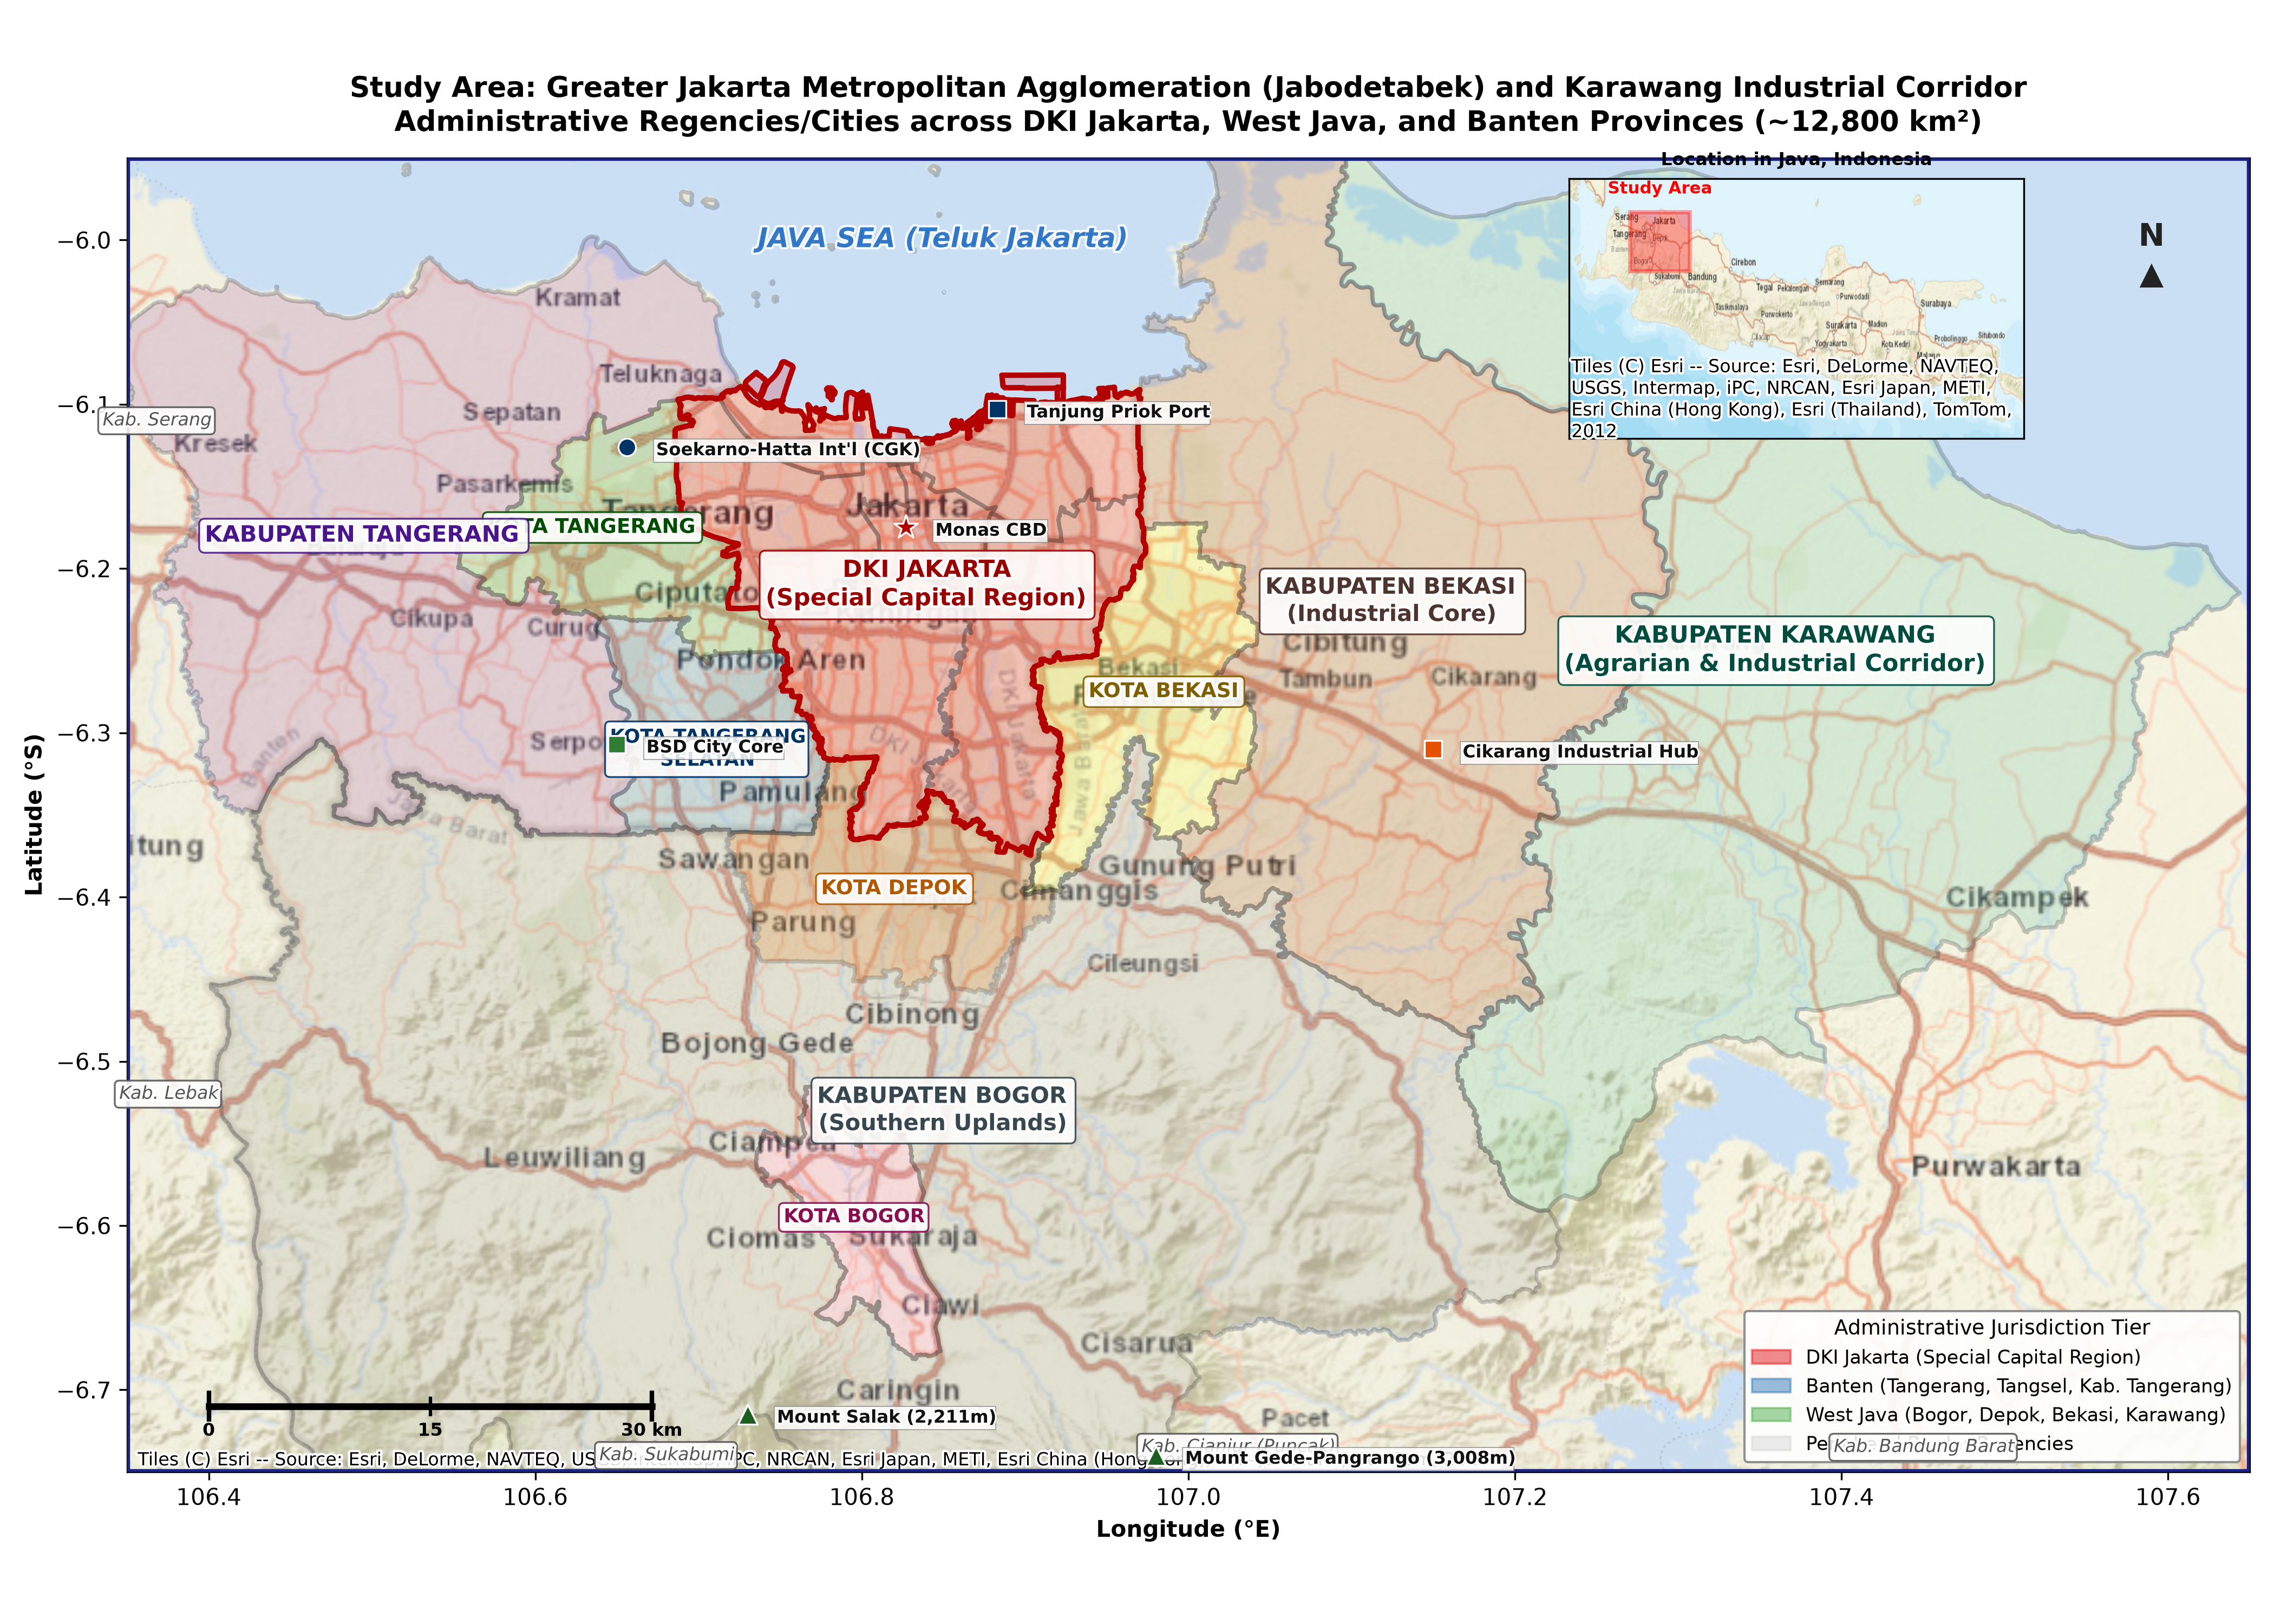
\includegraphics[width=0.98\textwidth]{../manuscript/figures/study_area_map.png}
\caption{Study area map encompassing Greater Jakarta (\textit{Jabodetabek}) and the Karawang industrial corridor ($\sim 9,800\text{ km}^2$), overlaid on an Esri WorldStreetMap basemap. Administrative boundaries delineate DKI Jakarta and constituent municipalities/regencies across Banten (Kota Tangerang, Kota Tangerang Selatan, Kabupaten Tangerang) and West Java (Kota Depok, Kota Bogor, Kabupaten Bogor, Kota Bekasi, Kabupaten Bekasi, Kabupaten Karawang). Major transportation hubs (CGK Airport, Tanjung Priok Port), commercial hubs (Monas CBD, BSD City, Cikarang), and southern volcanic landmarks (Mount Salak, Mount Gede) are indicated. Top-right inset highlights regional placement within Java Island, Indonesia.}
\label{fig:study_area_map}
\end{figure}

The study area is examined into equal-area hexagonal cells using the Uber H3 Discrete Global Grid System at \textbf{Resolution 8} ($0.737\text{ km}^2$).

\subsection{Multi-Source Dataset Inventory}
To capture the multi-dimensional physical reality of human living environments without local survey data, we harmonize 17 open-source multi-modal datasets spanning Earth observation satellites, airborne sensor models, continental building vector geometry, topological street graphs, gridded human settlement layers, and atmospheric chemical transport reanalysis. All dynamic observation layers are aligned to reference calendar year \textbf{2023} to eliminate mismatch condition due to temporal difference. Table~\ref{tab:dataset_inventory} provides an inventory of all datasets utilized across the research.

\begingroup
\small
\setlength{\tabcolsep}{3.5pt} % Tighten column padding (default is 6pt)
\renewcommand{\arraystretch}{1.15}

\begin{xltabular}{\textwidth}{
  >{\raggedright\arraybackslash}p{1.9cm}
  >{\raggedright\arraybackslash}p{2.1cm}
  >{\raggedright\arraybackslash}p{1.9cm}
  >{\centering\arraybackslash}p{1.2cm}
  >{\raggedright\arraybackslash}p{1.9cm}
  >{\raggedright\arraybackslash}p{1.8cm}
  >{\raggedright\arraybackslash}X
}
\caption{Comprehensive Multi-Source Dataset Inventory Across the Research Framework} \label{tab:dataset_inventory} \\
\toprule
\textbf{Category} & \textbf{Dataset} & \textbf{Source} & \textbf{Format} & \textbf{Resolution} & \textbf{Temporal Status} & \textbf{Research Relevance} \\
\midrule
\endfirsthead

\multicolumn{7}{c}{{\bfseries Table \thetable\ continued from previous page}} \\
\toprule
\textbf{Category} & \textbf{Dataset} & \textbf{Source} & \textbf{Format} & \textbf{Resolution} & \textbf{Temporal Status} & \textbf{Research Relevance} \\
\midrule
\endhead

\midrule
\multicolumn{7}{r}{\textit{Continued on next page}} \\
\bottomrule
\endfoot

\bottomrule
\endlastfoot

\textbf{Spatial Base} & Uber H3 DGGS (Res 8) & \href{https://h3geo.org/}{Uber Technologies} & Vector & 0.737 km$^2$ / 461 m & Static (v4.1) & Discrete global grid establishing equal-area, MAUP-invariant graph nodes ($N = 17,154$) for neural message passing. \\
\addlinespace
\textbf{Built Environment} & Google Open Buildings v3 & \href{https://sites.research.google/open-buildings/}{Google Research} & Vector & Footprints ($\ge 0.65$ conf) & 2023 release & Resolves building footprint geometries to compute total built footprint area and density. \\
\textbf{Built Environment} & Open Buildings 2.5D & \href{https://sites.research.google/open-buildings/}{Google Research} & Tabular / Model & Building-level / 100 m & 2023 annual composite & Predicts building floor counts to infer 3D living floor area per hexagon. \\
\textbf{Built Environment} & GHS-BUILT-S \& BUILT-C & \href{https://ghsl.jrc.ec.europa.eu/}{EC JRC} & Raster & 100 m & 2020 (interpolated 2023) & Distinguishes residential from industrial non-residential structures to isolate true living floor mass. \\
\addlinespace
\textbf{Demography} & JRC GHS-POP & \href{https://ghsl.jrc.ec.europa.eu/ghs_pop2023.php}{EC JRC} & Raster & 100 m & 2023 (interpolated) & Enumerates resident population (40.73M residents) to compute per-capita living space ($R_{\text{space}}$) and residential masks. \\
\textbf{Demography} & JRC GHS-SMOD & \href{https://ghsl.jrc.ec.europa.eu/ghs_smod2023.php}{EC JRC} & Raster & 1 km & 2020--2025 epoch & Degree of Urbanisation typology used to delineate urban centers, clusters, and rural reference cells. \\
\addlinespace
\textbf{Social Infrastructure} & Overture Maps Places & \href{https://overturemaps.org/}{Overture Maps} & Vector & Geocoded points & 2024-02-15 (for 2023) & Curated catalog of 173,820 daily necessities (markets, warungs, clinics, schools, worship) for walkability. \\
\textbf{Social Infrastructure} & OpenStreetMap Network & \href{https://download.geofabrik.de/asia/indonesia/java.html}{Geofabrik / OSM} & Vector & Network topology & 2024-01-01 snapshot & Pedestrian walking network for \texttt{city2graph} 15-minute topological Dijkstra isochrone routing. \\
\addlinespace
\textbf{Biophysical} & Sentinel-2 MSI L2A & \href{https://developers.google.com/earth-engine/datasets/catalog/COPERNICUS_S2_SR_HARMONIZED}{ESA / Copernicus} & Raster & 10 m / 20 m & Dry season 2023 (62 scenes) & Multi-spectral reflectance used to compute NDVI (canopy), NDBI (built density), and BSI (bare soil). \\
\textbf{Biophysical} & Dynamic World 10m & \href{https://developers.google.com/earth-engine/datasets/catalog/GOOGLE_DYNAMICWORLD_V1}{Google / WRI} & Raster & 10 m & 2023 (383 scenes) & High-resolution land cover probabilities to calculate surface water recurrence and validate canopy. \\
\textbf{Biophysical} & JRC Global Surface Water & \href{https://developers.google.com/earth-engine/datasets/catalog/JRC_GSW1_4_GlobalSurfaceWater}{EC JRC} & Raster & 30 m & Multi-decadal recurrence & Identifies permanent deep water bodies (marine bays, major lakes) to prevent distorted evaluations. \\
\addlinespace
\textbf{Microclimate} & Landsat 8/9 C2 L2 (ST\_B10) & \href{https://developers.google.com/earth-engine/datasets/catalog/LANDSAT_LC08_C02_T1_L2}{USGS / NASA} & Raster & 30 m & Dry season 2023 & Measures Land Surface Temperature (LST) and Surface Urban Heat Island ($\Delta\text{LST}$) above rural baseline. \\
\textbf{Microclimate} & MODIS Daily Daytime LST & \href{https://developers.google.com/earth-engine/datasets/catalog/MODIS_061_MOD11A1}{NASA LP DAAC} & Raster & 1,000 m & 2023 annual median & Independent thermodynamic cross-sensor sanity benchmark against Landsat 8/9 LST ($\rho = 0.882$). \\
\addlinespace
\textbf{Atmospheric Health} & ACAG V6.GL.02.04 $\text{PM}_{2.5}$ & \href{https://sites.wustl.edu/acag/datasets/surface-pm2-5/}{ACAG / WashU} & Raster & $0.01^\circ$ ($\sim$1.1 km) & 12 monthly grids (2023) & Fused satellite-chemical transport model reanalysis quantifying ambient ground-level fine particulate pollution. \\
\textbf{Atmospheric Health} & Sentinel-5P TROPOMI $\text{NO}_2$ & \href{https://developers.google.com/earth-engine/datasets/catalog/COPERNICUS_S5P_OFFL_L3_NO2}{ESA / Copernicus} & Raster & 1,113 m ($0.01^\circ$) & 2023 annual median & Quantifies tropospheric nitrogen dioxide combustion emissions along expressways and industrial corridors. \\
\textbf{Infrastructure} & NASA VIIRS Black Marble & \href{https://developers.google.com/earth-engine/datasets/catalog/NOAA_VIIRS_DNB_MONTHLY_V1_VCMCFG}{NASA LAADS DAAC} & Raster & 15 arc-sec ($\sim$464 m) & 2023 annual composite & Measures artificial nighttime luminosity to quantify nocturnal electrification and commercial energy density. \\
\addlinespace
\textbf{Socioeconomic Valid.} & Meta Relative Wealth Index & \href{https://data.humdata.org/dataset/relative-wealth-index}{Meta Data for Good} & Vector & 2.4 km micro-tiles & 2021 release & Supervised survey asset wealth baseline used in 4-quadrant divergence analysis against physical standards. \\
\textbf{Socioeconomic Valid.} & BPS Municipal Statistics & \href{https://www.bps.go.id/}{BPS Indonesia} & Tabular & Regency / District & 2023 annual releases & Official municipal poverty rates, density, and socioeconomic census data for macro-regional benchmarking. \\
\textbf{Ground-Truth Valid.} & Official Slum Decrees & \href{https://kotaku.pu.go.id/}{Bappeda / PUPR} & Vector & Sub-neighborhood & 2020--2023 decrees & Delineates surveyed informal settlements (\textit{RW Kumuh}) for spatial validation of detected segregation edges. \\
\end{xltabular}
\endgroup

\subsection{Ten-Dimensional Physical Feature Engineering and Universal Baselines}
To eliminate localized normalization stretching where scores cannot be ported across cities, indicators are standardized against \textbf{Universal Frozen Physical Benchmarks} anchored to international shelter, environmental health, and pedestrian accessibility guidelines (UN-Habitat shelter area threshold of $9.0\text{ m}^2/\text{capita}$, WHO clean air guidelines of $5.0\ \mu\text{g}/\text{m}^3$, and 15-minute walking catchments; Table~\ref{tab:benchmarks}).

\begin{table}[htbp]
\centering
\small
\setlength{\tabcolsep}{4.5pt}
\renewcommand{\arraystretch}{1.15}
\caption{Universal 10-Dimensional Physical Living Standard Benchmark Parameters}
\label{tab:benchmarks}
\begin{tabularx}{\textwidth}{
  c
  >{\raggedright\arraybackslash}X
  >{\raggedright\arraybackslash}p{2.8cm}
  >{\raggedright\arraybackslash}p{2.3cm}
  c
  c
}
\toprule
\textbf{Index} & \textbf{Dimension Name} & \textbf{Raw Unit} & \textbf{Transformation} & \textbf{Lower ($L_k$)} & \textbf{Upper ($U_k$)} \\
\midrule
$X_1$    & Space Sufficiency ($R_{\text{space}}$)        & Floor area per capita                        & None            & $0.0$               & $6.0$ ($54\text{ m}^2$) \\
$X_2$    & Built-up Density (NDBI)                       & Spectral Index                               & None            & $-0.50$             & $+0.30$                 \\
$X_3$    & Walkable Amenities ($A_{\text{amenity}}$)     & 15-min POI Count                             & $\log(1 + x)$   & $0.0$               & $\log(501) \approx 6.22$ \\
$X_4$    & Bare Soil / Dust (BSI)                        & Spectral Index                               & None            & $-0.40$             & $+0.30$                 \\
$X_5$    & Nighttime Energy (VIIRS)                      & $\text{nW}\cdot\text{cm}^{-2}\cdot\text{sr}^{-1}$ & $\log(1 + x)$   & $0.0$               & $\log(101) \approx 4.62$ \\
$X_6$    & Canopy Greenness (NDVI)                       & Spectral Index                               & None            & $-0.10$             & $+0.80$                 \\
$X_7$    & Thermal Comfort ($\Delta\text{LST}_{\text{inv}}$) & Kelvin above rural                       & None            & $-5.0\text{ K}$     & $+15.0\text{ K}$        \\
$X_8$    & Surface Water Frequency                       & Fraction $[0, 1]$                            & None            & $0.00$              & $1.00$                  \\
$X_9$    & Particulate Purity ($\text{PM25}_{\text{inv}}$) & $\mu\text{g}/\text{m}^3$                   & None            & $5.0$               & $100.0$                 \\
$X_{10}$ & Nitrogen Dioxide ($\text{NO2}_{\text{inv}}$)  & $\text{mol}/\text{m}^2$                      & None            & $0.0$               & $2.5 \times 10^{-4}$    \\
\bottomrule
\end{tabularx}
\end{table}

Filtering by residential criteria ($\text{Pop} \ge 300/\text{cell}$, $\text{Buildings} \ge 1$, $\text{SMOD} \in \{21, 22, 23, 30\}$) isolates \textbf{$N_{\text{res}} = 9,345$ residential cells} ($54.5\%$ of territory, housing the entire 40.73M population), of which \textbf{$N_{\text{modelled}} = 7,943$ cells} possess complete satellite observations across all 10 channels. The remaining cells are retained in the spatial adjacency graph ($|E| = 101,848$ edges) to preserve topological contiguity for Graph Attention Autoencoder message passing.

\section{Methodology}
\begin{itemize}[leftmargin=*]
    \item \textbf{Multi-dimensional Feature Harmonization}
    \begin{itemize}
        \item Living space sufficiency. Ratio of floor area per capita (building footprint * building level / population) measured against international minimum standard.
        \item Cumulative 15-minutes accessibility to amenities
        \item Built-up density via NDBI spectral index
        \item Unpaved street (BSI) index
        \item Economic radiance, illumation at night from VIIRS
        \item Vegetation density via NDVI
        \item Temperature comfort via LST
        \item Water exposure via NDWI
        \item PM25 pollution
        \item Broad air quality index (AQI)
    \end{itemize}
    \item \textbf{Graph Attention Autoencoder (GAT-AE)}
    \begin{itemize}
        \item Analyze spatial autocorrelation of the multidimensional features
        \item Derive the disparity index
        \item Analyze the friction between low and high scoring areas
    \end{itemize}
    \item \textbf{Neighborhood typology}
    \begin{itemize}
        \item What kind of living standard do we have for each pixel? Need machine learning-based clustering method
        \item Possible to calculate something like a local palma or gini ratio for inequality analysis? Maybe, but optional
    \end{itemize}
    \item \textbf{Validation}
    \begin{itemize}
        \item Fetch low-scoring areas in Greater Jakarta, overlap with KOTAKU slum survey as reference data
    \end{itemize}
\end{itemize}

\section{Results}
Placeholder...

\section{Discussion}
Placeholder...

\section{Conclusion}
\begin{itemize}[leftmargin=*]
    \item Summary of the open-science GeoAI pipeline.
    \item Global transferability across rapidly urbanizing Global South metropolitan regions.
\end{itemize}

\end{document}